\label{s:hz}
\subsection{Potentially Rocky Planets in the Habitable Zone}
In order for this catalog to be used to understand the occurrence of rocky exoplanets in the habitable zone of sun-like stars, it needs to identify small, temperate candidates around G-dwarf stars.  The DR25 catalog uses the transit depth and the period, along with the DR25 stellar table \citet{Mathur2017ApJS}, to derive the planet radius and the semi-major axis of the planet's orbit.  From these we calculate the insolation flux relative to the insolation flux of the earth:

\begin{equation}
S_{p} = \frac{R_{p}^{2} \cdot (T_{\star}/5777)^{4}}{a^{2}}
\end{equation}

\noindent where $a$ is the semi-major axis of the planet's orbit in AU, \tstar{} is in Kelvin, 5777~K is the effective temperature of the Sun, and \sp{} and \rp{} are in Earth units. The errors for both insolation flux and radii include the errors from the DR25 stellar catalog. 

In Table~\ref{t:hz} we highlight the DR25 catalog candidates that are potentially terrestrial and fall in or near the habitable zone of their star.  We select these stars to be any candidate whose one sigma error bars indicate the radius could be smaller than 1.8 \re, and the insolation flux is within the optimistic habitable zone defined by the wide habitable zone of \citet{Kopparapu2013}.  We also only show those with a disposition score above 0.5.  We chose this disposition score threshold because estimates of the reliability of these candidates, even for those around G dwarf stars, is greater than 80 per cent.  This produces XX46XX candidates in the DR25 catalog. Of these, 10 are new to the DR25 catalog. We plot these candidates in Figure~\ref{f:hzNarrow}.  A manual review of the 10 new high-score candidates indicates that they are primarily low signal-to-noise, with very few transits, but show no obvious reason to be called a false positive. In order to make Table~\ref{t:hz} complete we also include any terrestrial-sized confirmed planet that falls in the habitable zone of its star according to the confirmed planet table at NExScI, see the footnotes. The objects are included even if the DR25 catalog calls it a false positive or if the DR25 planetary parameters place it outside the habitable zone. Table~ref{t:hz} and Figure~\ref{f:hzNarrow} give the DR25 catalog planetary values.



%The reliability measurements for this catalog indicate that for long period, low MES objects (which applies to all those on this plot found on a star with a temperature above 5000\,K) and a disposition score cut greater than 0.5, the reliability is $\approx$80XX per cent, see \S\ref{s:reliability}. 



\begin{figure}
    \centering
    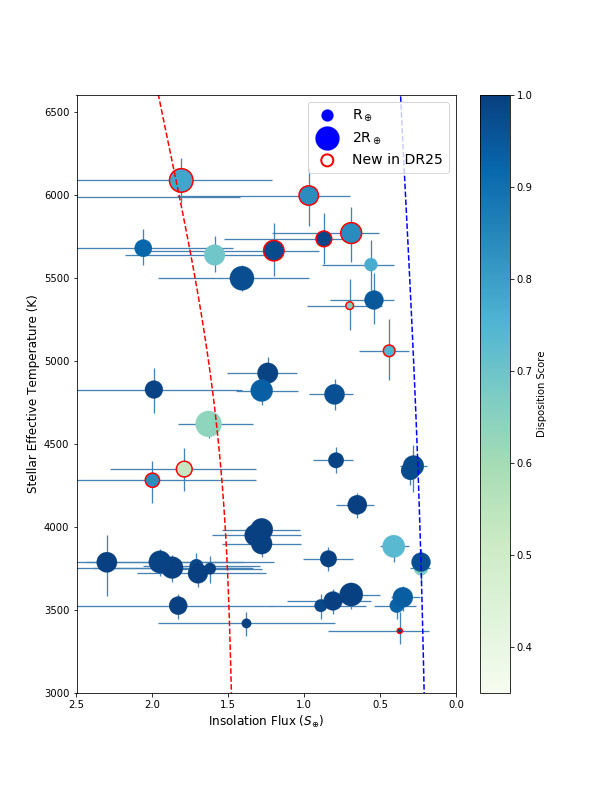
\includegraphics[width=1.1\linewidth]{fig-hzTstarInsol.png}
    \caption{DR25 Exoplanet Candidates plotted as stellar effective temperature against insolation flux. The size of the exoplanet is indicated by the size of the circle.  The color indicates the disposition score. Only those with disposition score greater than 0.5 are plotted.  Only objects whose error bars indicate that they could be in the habitable zone and have a radii less than 1.8\re are shown. Those with a magenta ring are new to the DR25 catalog. }
    \label{f:hzNarrow}
\end{figure}


\clearpage
%\LongTables

\begin{deluxetable*}{rrlrrrrrrr}
\tablecolumns{10}
\tabletypesize{\scriptsize}
\tablewidth{\linewidth}
\tablecaption{Habitable Zone Planet Candidates}
\tablehead{
\colhead{KOI} &
\colhead{KIC} &
\colhead{Kepler} &
\colhead{Period} &
\colhead{\rp} &
\colhead{\sp} &
\colhead{\tstar} &
\colhead{\rstar} &
\colhead{MES} &
\colhead{Score} \\ 
\colhead{} &
\colhead{} &
\colhead{} &
\colhead{[days]} &
\colhead{[\re]} &
\colhead{[\se]} &
\colhead{[K]} &
\colhead{[\rsun]} 
}
\startdata
172.02 & 8692861 & Kepler-69 c & 242.46130 & 1.73$^{+0.21}_{-0.22}$ & 1.59$^{+0.59}_{-0.45}$ & 5637$^{+113}_{-101}$ & 0.94$^{+0.12}_{-0.12}$ & 18.0 & 0.693 \\ 
238.03 & 7219825 & \nodata & 362.97828 & 1.96$^{+0.33}_{-0.29}$ & 1.81$^{+0.87}_{-0.60}$ & 6086$^{+133}_{-133}$ & 1.22$^{+0.20}_{-0.18}$ & 11.9 & 0.784 \\ 
438.02 & 12302530 & Kepler-155 c & 52.66153 & 1.87$^{+0.11}_{-0.12}$ & 1.28$^{+0.26}_{-0.25}$ & 3984$^{+71}_{-86}$ & 0.54$^{+0.03}_{-0.04}$ & 30.6 & 1.000 \\ 
463.01\tablenotemark{c} & 8845205 & Kepler-560 b & 18.47763 & 1.55$^{+0.32}_{-0.29}$ & 1.21$^{+0.72}_{-0.47}$ & 3395$^{+74}_{-67}$ & 0.28$^{+0.06}_{-0.05}$ & 78.0 & 0.001 \\ 
494.01 & 3966801 & Kepler-577 b & 25.69581 & 1.70$^{+0.21}_{-0.33}$ & 2.30$^{+1.17}_{-1.10}$ & 3787$^{+163}_{-204}$ & 0.48$^{+0.06}_{-0.09}$ & 35.9 & 1.000 \\ 
571.05\tablenotemark{a} & 8120608 & Kepler-186 f & 129.94410 & 1.18$^{+0.11}_{-0.14}$ & 0.23$^{+0.07}_{-0.06}$ & 3751$^{+75}_{-84}$ & 0.44$^{+0.04}_{-0.05}$ & 7.7 & 0.677 \\ 
701.03 & 9002278 & Kepler-62 e & 122.38740 & 1.72$^{+0.10}_{-0.07}$ & 1.24$^{+0.27}_{-0.19}$ & 4926$^{+98}_{-98}$ & 0.66$^{+0.04}_{-0.03}$ & 35.9 & 0.994 \\ 
701.04\tablenotemark{d} & 9002278 & Kepler-62 f & 267.29100 & 1.43$^{+0.08}_{-0.06}$ & 0.44$^{+0.09}_{-0.07}$ & 4926$^{+98}_{-98}$ & 0.66$^{+0.04}_{-0.03}$ & 14.3 & 0.000 \\ 
812.03 & 4139816 & Kepler-235 e & 46.18420 & 1.83$^{+0.12}_{-0.15}$ & 1.32$^{+0.29}_{-0.30}$ & 3950$^{+70}_{-86}$ & 0.49$^{+0.03}_{-0.04}$ & 18.0 & 1.000 \\ 
854.01 & 6435936 & Kepler-705 b & 56.05608 & 1.94$^{+0.12}_{-0.22}$ & 0.69$^{+0.15}_{-0.19}$ & 3593$^{+71}_{-86}$ & 0.49$^{+0.03}_{-0.06}$ & 19.3 & 0.996 \\ 
947.01 & 9710326 & Kepler-737 b & 28.59914 & 1.83$^{+0.16}_{-0.21}$ & 1.87$^{+0.52}_{-0.53}$ & 3755$^{+75}_{-84}$ & 0.46$^{+0.04}_{-0.05}$ & 45.7 & 1.000 \\ 
1078.03 & 10166274 & Kepler-267 d & 28.46465 & 1.87$^{+0.14}_{-0.22}$ & 1.95$^{+0.49}_{-0.55}$ & 3789$^{+75}_{-82}$ & 0.46$^{+0.04}_{-0.05}$ & 22.2 & 0.992 \\ 
1298.02\tablenotemark{d} & 10604335 & Kepler-283 c & 92.74958 & 1.87$^{+0.08}_{-0.10}$ & 0.78$^{+0.15}_{-0.14}$ & 4141$^{+83}_{-91}$ & 0.58$^{+0.03}_{-0.03}$ & 10.7 & 0.000 \\ 
1404.02 & 8874090 & \nodata & 18.90609 & 0.87$^{+0.16}_{-0.21}$ & 3.03$^{+2.29}_{-1.67}$ & 3751$^{+219}_{-219}$ & 0.45$^{+0.08}_{-0.11}$ & 10.1 & 0.955 \\ 
1422.02 & 11497958\tablenotemark{b} & Kepler-296 d & 19.85029 & 1.52$^{+0.19}_{-0.23}$ & 1.83$^{+0.68}_{-0.62}$ & 3526$^{+71}_{-78}$ & 0.38$^{+0.05}_{-0.06}$ & 25.1 & 1.000 \\ 
1422.04 & 11497958 & Kepler-296 f & 63.33627 & 1.18$^{+0.15}_{-0.18}$ & 0.39$^{+0.15}_{-0.13}$ & 3526$^{+71}_{-78}$ & 0.38$^{+0.05}_{-0.06}$ & 9.1 & 0.927 \\ 
1422.05 & 11497958 & Kepler-296 e & 34.14211 & 1.06$^{+0.13}_{-0.16}$ & 0.89$^{+0.33}_{-0.30}$ & 3526$^{+71}_{-78}$ & 0.38$^{+0.05}_{-0.06}$ & 10.5 & 0.984 \\ 
1596.02 & 10027323 & Kepler-309 c & 105.35823 & 1.87$^{+0.13}_{-0.17}$ & 0.41$^{+0.09}_{-0.10}$ & 3883$^{+69}_{-93}$ & 0.50$^{+0.04}_{-0.04}$ & 16.5 & 0.738 \\ 
2162.02 & 9205938 & \nodata & 199.66876 & 1.45$^{+0.18}_{-0.18}$ & 2.06$^{+0.76}_{-0.59}$ & 5678$^{+113}_{-102}$ & 0.92$^{+0.12}_{-0.12}$ & 11.1 & 0.920 \\ 
2418.01 & 10027247 & Kepler-1229 b & 86.82952 & 1.68$^{+0.12}_{-0.21}$ & 0.35$^{+0.08}_{-0.11}$ & 3576$^{+71}_{-85}$ & 0.46$^{+0.03}_{-0.06}$ & 11.7 & 0.937 \\ 
2626.01 & 11768142 & \nodata & 38.09707 & 1.58$^{+0.20}_{-0.21}$ & 0.81$^{+0.30}_{-0.25}$ & 3554$^{+71}_{-80}$ & 0.40$^{+0.05}_{-0.05}$ & 14.6 & 0.999 \\ 
2650.01 & 8890150 & Kepler-395 c & 34.98978 & 1.14$^{+0.07}_{-0.10}$ & 1.71$^{+0.35}_{-0.42}$ & 3765$^{+75}_{-83}$ & 0.52$^{+0.03}_{-0.05}$ & 10.1 & 0.985 \\ 
2719.02 & 5184911 & \nodata & 106.25976 & 1.50$^{+0.10}_{-0.16}$ & 1.99$^{+0.53}_{-0.58}$ & 4827$^{+129}_{-144}$ & 0.82$^{+0.06}_{-0.09}$ & 10.0 & 0.990 \\ 
3010.01 & 3642335 & Kepler-1410 b & 60.86610 & 1.39$^{+0.07}_{-0.10}$ & 0.84$^{+0.17}_{-0.16}$ & 3808$^{+69}_{-76}$ & 0.52$^{+0.03}_{-0.04}$ & 12.7 & 0.996 \\ 
3034.01 & 2973386 & \nodata & 31.02092 & 1.66$^{+0.12}_{-0.17}$ & 1.70$^{+0.40}_{-0.45}$ & 3720$^{+73}_{-81}$ & 0.48$^{+0.03}_{-0.05}$ & 11.9 & 1.000 \\ 
3138.01\tablenotemark{b} & 6444896 & Kepler-1649 b & 8.68909 & 0.49$^{+0.00}_{-0.00}$ & 0.47$^{+0.00}_{-0.00}$ & 2703$^{+0}_{-0}$ & 0.12$^{+0.00}_{-0.00}$ & 12.0 & 1.000 \\ 
3282.01 & 12066569 & Kepler-1455 b & 49.27684 & 1.75$^{+0.09}_{-0.13}$ & 1.28$^{+0.26}_{-0.26}$ & 3899$^{+78}_{-78}$ & 0.53$^{+0.03}_{-0.04}$ & 14.7 & 0.996 \\ 
3284.01 & 6497146 & Kepler-438 b & 35.23319 & 0.97$^{+0.06}_{-0.07}$ & 1.62$^{+0.37}_{-0.34}$ & 3749$^{+75}_{-84}$ & 0.52$^{+0.03}_{-0.04}$ & 11.9 & 1.000 \\ 
3497.01 & 8424002 & Kepler-1512 b & 20.35972 & 0.80$^{+0.12}_{-0.16}$ & 1.38$^{+0.58}_{-0.58}$ & 3419$^{+67}_{-76}$ & 0.34$^{+0.05}_{-0.07}$ & 19.6 & 1.000 \\ 
4005.01\tablenotemark{a} & 8142787 & Kepler-439 b & 178.13960 & 2.25$^{+0.22}_{-0.16}$ & 1.70$^{+0.47}_{-0.31}$ & 5431$^{+81}_{-81}$ & 0.88$^{+0.09}_{-0.06}$ & 17.8 & 0.997 \\ 
4036.01 & 11415243 & Kepler-1544 b & 168.81133 & 1.69$^{+0.10}_{-0.06}$ & 0.80$^{+0.17}_{-0.12}$ & 4798$^{+95}_{-95}$ & 0.71$^{+0.04}_{-0.03}$ & 14.8 & 0.965 \\ 
4087.01 & 6106282 & Kepler-440 b & 101.11141 & 1.61$^{+0.10}_{-0.08}$ & 0.65$^{+0.14}_{-0.11}$ & 4133$^{+74}_{-82}$ & 0.56$^{+0.03}_{-0.03}$ & 15.7 & 1.000 \\ 
4356.01\tablenotemark{a} & 8459663 & Kepler-1593 b & 174.51028 & 1.74$^{+0.14}_{-0.20}$ & 0.28$^{+0.09}_{-0.09}$ & 4367$^{+124}_{-155}$ & 0.45$^{+0.04}_{-0.05}$ & 11.0 & 0.976 \\ 
4427.01 & 4172805 & \nodata & 147.66173 & 1.59$^{+0.12}_{-0.14}$ & 0.23$^{+0.06}_{-0.05}$ & 3788$^{+76}_{-84}$ & 0.49$^{+0.04}_{-0.04}$ & 10.8 & 0.969 \\ 
4460.01 & 9947389 & \nodata & 284.72721 & 2.02$^{+0.30}_{-0.29}$ & 1.41$^{+0.55}_{-0.44}$ & 5497$^{+82}_{-74}$ & 1.08$^{+0.16}_{-0.16}$ & 10.7 & 0.972 \\ 
4550.01 & 5977470 & \nodata & 140.25194 & 1.84$^{+0.05}_{-0.12}$ & 1.28$^{+0.17}_{-0.24}$ & 4821$^{+76}_{-86}$ & 0.79$^{+0.02}_{-0.05}$ & 9.6 & 0.934 \\ 
4622.01 & 11284772 & Kepler-441 b & 207.24820 & 1.56$^{+0.09}_{-0.06}$ & 0.30$^{+0.06}_{-0.05}$ & 4339$^{+78}_{-87}$ & 0.55$^{+0.03}_{-0.02}$ & 9.7 & 0.975 \\ 
4742.01 & 4138008 & Kepler-442 b & 112.30530 & 1.30$^{+0.07}_{-0.05}$ & 0.79$^{+0.15}_{-0.11}$ & 4401$^{+78}_{-78}$ & 0.59$^{+0.03}_{-0.02}$ & 12.9 & 0.993 \\ 
7016.01 & 8311864 & Kepler-452 b & 384.84300 & 1.09$^{+0.20}_{-0.10}$ & 0.56$^{+0.32}_{-0.15}$ & 5579$^{+150}_{-150}$ & 0.80$^{+0.15}_{-0.07}$ & 7.6 & 0.771 \\ 
7223.01 & 9674320 & \nodata & 317.06242 & 1.59$^{+0.27}_{-0.12}$ & 0.54$^{+0.29}_{-0.13}$ & 5366$^{+160}_{-144}$ & 0.71$^{+0.12}_{-0.05}$ & 10.3 & 0.947 \\ 
7706.01 & 4762283 & \nodata & 42.04952 & 1.19$^{+0.08}_{-0.16}$ & 2.00$^{+0.55}_{-0.68}$ & 4281$^{+115}_{-140}$ & 0.48$^{+0.03}_{-0.06}$ & 7.5 & 0.837 \\ 
7711.01 & 4940203 & \nodata & 302.77982 & 1.31$^{+0.34}_{-0.12}$ & 0.87$^{+0.66}_{-0.22}$ & 5734$^{+154}_{-154}$ & 0.80$^{+0.21}_{-0.07}$ & 8.5 & 0.987 \\ 
7882.01 & 8364232 & \nodata & 65.41518 & 1.31$^{+0.08}_{-0.12}$ & 1.79$^{+0.49}_{-0.47}$ & 4348$^{+130}_{-130}$ & 0.65$^{+0.04}_{-0.06}$ & 7.2 & 0.529 \\ 
7894.01 & 8555967 & \nodata & 347.97611 & 1.62$^{+0.49}_{-0.15}$ & 0.97$^{+0.87}_{-0.27}$ & 5995$^{+163}_{-181}$ & 0.88$^{+0.27}_{-0.08}$ & 8.5 & 0.837 \\ 
7923.01 & 9084569 & \nodata & 395.13138 & 0.97$^{+0.12}_{-0.10}$ & 0.44$^{+0.20}_{-0.13}$ & 5060$^{+192}_{-174}$ & 0.87$^{+0.10}_{-0.09}$ & 10.0 & 0.750 \\ 
%7938.01 & 9469494 & \nodata & 275.56030 & 2.33$^{+0.53}_{-1.32}$ & 8.60$^{+6.29}_{-7.18}$ & 5989$^{+213}_{-192}$ & 2.47$^{+0.56}_{-1.40}$ & 7.5 & 0.508 \\ 
7954.01 & 9650762 & \nodata & 372.15035 & 1.74$^{+0.46}_{-0.14}$ & 0.69$^{+0.52}_{-0.18}$ & 5769$^{+155}_{-172}$ & 0.81$^{+0.21}_{-0.07}$ & 8.9 & 0.839 \\ 
8000.01 & 10331279 & \nodata & 225.48805 & 1.70$^{+0.43}_{-0.14}$ & 1.20$^{+0.90}_{-0.30}$ & 5663$^{+169}_{-152}$ & 0.78$^{+0.19}_{-0.07}$ & 8.7 & 0.975 \\ 
8012.01 & 10452252 & \nodata & 34.57372 & 0.42$^{+0.17}_{-0.12}$ & 0.37$^{+0.47}_{-0.19}$ & 3374$^{+112}_{-82}$ & 0.22$^{+0.09}_{-0.06}$ & 7.7 & 0.989 \\ 
8174.01 & 8873873 & \nodata & 295.06066 & 0.64$^{+0.07}_{-0.07}$ & 0.70$^{+0.28}_{-0.21}$ & 5332$^{+160}_{-144}$ & 0.76$^{+0.09}_{-0.09}$ & 7.4 & 0.665 \\ 
\enddata
\label{hzearthstab}
\tablenotetext{a}{Confirmed planet properties from NASA Exoplanet Archive on May 31, 2017 place object inside HZ.}
\tablenotetext{b}{Confirmed planet properties from NASA Exoplanet Archive on May 31, 2017 place object outside HZ.}
\tablenotetext{c}{Confirmed planet with vetting score less than 0.5.}
\tablenotetext{d}{Confirmed planet dispositioned as False Positive in DR25.}
\end{deluxetable*}


%See Figure~\ref{f:hzPlot} for a plot of planet radius against insolation flux at the small, cool end of the DR25 catalog. On this figure the color indicates the stellar temperature and the size of the point indicates the disposition score.  Notice that this part of the catalog is dominated by K and M stars despite the fact that the exoplanet search targets G stars \citet{Batalha2010}.

%\begin{figure*}
%    \centering
%    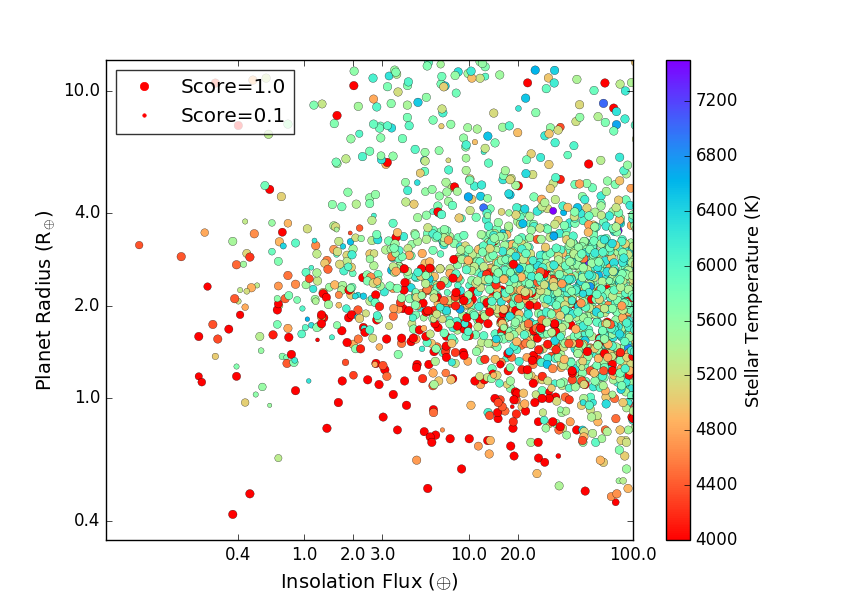
\includegraphics[width=1.1\linewidth]{fig-CatalogRadiusInsolScore.png}
%    \caption{DR25 Exoplanet Candidates plotted as planet radius against Insolation Flux, %in units of the flux that the Earth receives from the Sun. The stellar temperature is given by the color of the circle and the size of the circle indicates the Disposition Score. The planet radii are derived from the MCMC fits. }
%    \label{f:hzPlot}
%\end{figure*}